%!TEX root = thesis.tex

\chapter{Einleitung}

Das Ausleihen von Assets jeglicher Art ist keine Neuheit \todo{Söderholm}. An der Zentralen
Hochschulbibliothek Lübeck (ZHB) wird die Buchungsapp \textit{Affluences} verwendet. Zum Ausleihen von
Materialien, müssen Terminabholungen online gebucht werden \todo{(ZHB, o. J.)}. Die Anfragen können
überprüft werden, wodurch das vorausschauende Planen der Materialien ermöglicht wird. Am \ac{imis}
werden Assets ohne Anmeldung oder mit einer mündlichen Absprache verwendet. Aufseiten der
Mitarbeitenden wird der Gebrauch der Assets individuell geplant, sodass das frühzeitige Reservieren
oder das geplante Ausleihen erschwert wird. Für die vorausschauende Planung von anstehenden
Projekten gibt es keinerlei feste Reservierung oder einen Überblick, wann die gewünschten Assets
wieder verfügbar sind. Zudem ist vielen Mitarbeitenden unklar, welche Assets sich in den Laboren des
\ac{imis} befinden. Folglich kennen Mitarbeitende nur selten die Möglichkeiten, mit denen sie ihre
Forschungsprojekte oder die Lehre ergänzen könnten.

Aktuell werden Reservierungen sowie der Gebrauch von Equipment über unterschiedliche
Kommunikationswege wie E-Mail oder direkte Absprache bei zuständigen Mitarbeitenden angefragt. Die
zuständigen Mitarbeitenden prüfen die Anfrage und koordinieren potenzielle Kollisionen mit bereits
reservierten Zeiträumen oder Absprachen und bestätigen, ändern oder lehnen die
(Reservierungs-)Anfrage ab. In einigen Fällen werden die gebuchten Zeiten auf Papier dokumentiert.
Aufseiten der Studierenden kann ein solches System für Gruppenarbeiten, wie zum Beispiel die des Moduls
„Einführung in die Medieninformatik“ hilfreich sein. Studierende müssen während dieses Projekts eine
multimediale Abgabe produzieren, welche beispielsweise die Form eines Videos haben kann. Aktuell ist
vielen Studierenden nicht bewusst, dass das \ac{imis} Equipment wie Kameras, Greenscreen oder Gimbal für
Videos bereitstellt. Des Weiteren sind Hemmschwelle und Aufwand zum Ausleihen der Hardware hoch, da
uneindeutig ist, welche Mitarbeitenden für die jeweilige Hardware zuständig sind.


\section{Ziel der Arbeit}
Das Ziel dieser Arbeit ist es ein wirksames System zu entwickeln, welches den Reservierungs- und
Entleihprozess am \ac{imis} einheitlicher, effizienter und zufriedenstellender lösen lässt. Die
Anwendung soll es unter anderem ermöglichen, die auszuleihenden Assets in einer Liste abzubilden und
diese zu durchsuchen. In diesem Zusammenhang soll auch das Anzeigen einer Stückzahl der jeweils
verfügbaren Assets, deren Bedienungsanleitung sowie die verantwortlichen Mitarbeitenden umgesetzt
werden. Das Reservierungstool soll eine niedrigschwellige Möglichkeit bieten, um Mitarbeitenden die
Arbeit im Reservierungsprozess zu erleichtern. Außerdem soll es eine Übersicht über Utensilien
geben, sodass Mitarbeitende nicht mehr im Unklaren über die Hardware-Möglichkeiten sind und das
Material optimal ausgelastet werden kann.

Die Basis für ein solches Tool schafft die Asset Managementsoftware \textit{Snipe-IT}
\cite{noauthor_home_nodate}, welche bereits am \ac{imis} eingesetzt wird. \textit{Snipe-IT} ist eine
kostenlose, quelloffene IT-Asset-Verwaltungs-Plattform, welche das Nachverfolgen von
Software-Lizenzen, Hardware und Verbrauchsgegenständen ermöglicht. Genannte Assets können über ein
Dashboard hinzugefügt, verwaltet und gelöscht werden. Über Labels können Assets zur
Übersichtlichkeit in verschiedene Kategorien eingeordnet werden, während Tags ein Asset eindeutig
identifizieren (z. B. Seriennummer). Zudem ermöglicht das „Checkin/Checkout“-System die
Nachverfolgung aller Assets, falls diese zum Beispiel an Person ausgeliehen werden. Zu jedem
Zeitpunkt kann ein Asset maximal einer Person zugeordnet werden, wodurch das mehrfache gleichzeitige
Ausleihen eines Assets verhindert wird. Da \textit{Snipe-IT} selbst die zukünftige Reservierung
nicht unterstützt, umfasst das Ziel der Arbeit ein \textit{Snipe-IT Companion}, welcher das
Ausleihen in die Zukunft möglich macht.


\section{Forschungsfragen}
Im Sinne der eingangs beschriebenen Ziele soll im Rahmen der vorliegenden Arbeit untersucht werden,
wie ein Reservierungstool gestaltet werden kann, um Mitarbeitenden und Studierenden darin zu
unterstützen, Assets einsehen und ausleihen zu können.

Um den aktuellen Stand und die Probleme des aktuellen Ausleihprozess nachvollziehen zu können,
müssen diese zunächst ermittelt und klassifiziert werden. Die erste Forschungsfrage beschäftigt sich
daher mit der Analyse der Schwierigkeit des Ausleihprozesses.
\begin{enumerate}
  \item[\sffamily\color{maincolor} {F1 |}] {Welche zentralen Schwierigkeiten bringt die aktuelle Planung und Reservierung von Assets für Mitarbeitende und Studierende mit sich?}
\end{enumerate}

Um die zentralen Schwierigkeiten und Probleme lösen zu können, müssen Anforderungen an das System
ermittelt werden. Anschließend müssen diese nach Relevanz sortiert werden, um möglichst viele
Schwierigkeiten lösen zu können. Die zweite Forschungsfrage beschäftigt sich folglich mit den
Anforderungen, welche ein solches Reservierungstool umfassen sollte, um die Schwierigkeiten zu minimieren.

\begin{enumerate}
  \item[\sffamily\color{maincolor} {F2 |}] {Was sind Anforderungen an ein System, welches die in F1 gezeigten Schwierigkeiten adressiert und reduziert?}
\end{enumerate}

Abschließend soll eruiert werden, ob die erste Iteration des Systems die ermittelten Schwierigkeiten
mit den erarbeiteten Funktionalitäten lösen kann. Die letzte Forschungsfrage beschäftigt sich
demzufolge mit der Evaluation des erarbeiteten Systems und den möglichen stärken und schwächen.

\begin{enumerate}
  \item[\sffamily\color{maincolor} {F3 |}] {Inwieweit kann ein aus F2 resultierender Prototyp die in F1 identifizierten Schwierigkeit reduzieren?}
\end{enumerate}

\section{Vorgehensweise}
Die Entwicklung des Systems orientiert sich am menschenzentrierten Gestaltungsprozess
\cite{din_en_iso_9421-2102020-03_din_nodate}. Der Prozess teilt sich im Rahmen dieser Arbeit in
fünf aufeinanderfolgende Phasen {\ref{fig:schablone}} wobei die Entwurfs- und Implementierungsphasen
Spielraum für ein iteratives Vorgehen lassen. Unter anderem werden in der Analyse die Aufgaben des
Systems, die Benutzenden und der Kontext nach dem Entwicklungsprozess für interaktive Medien
\cite{herczeg_einfuhrung_2009} aufgeführt, um ein gebrauchstaugliches Ergebnis erzielen zu können.

\begin{figure}[h]
  \centering
  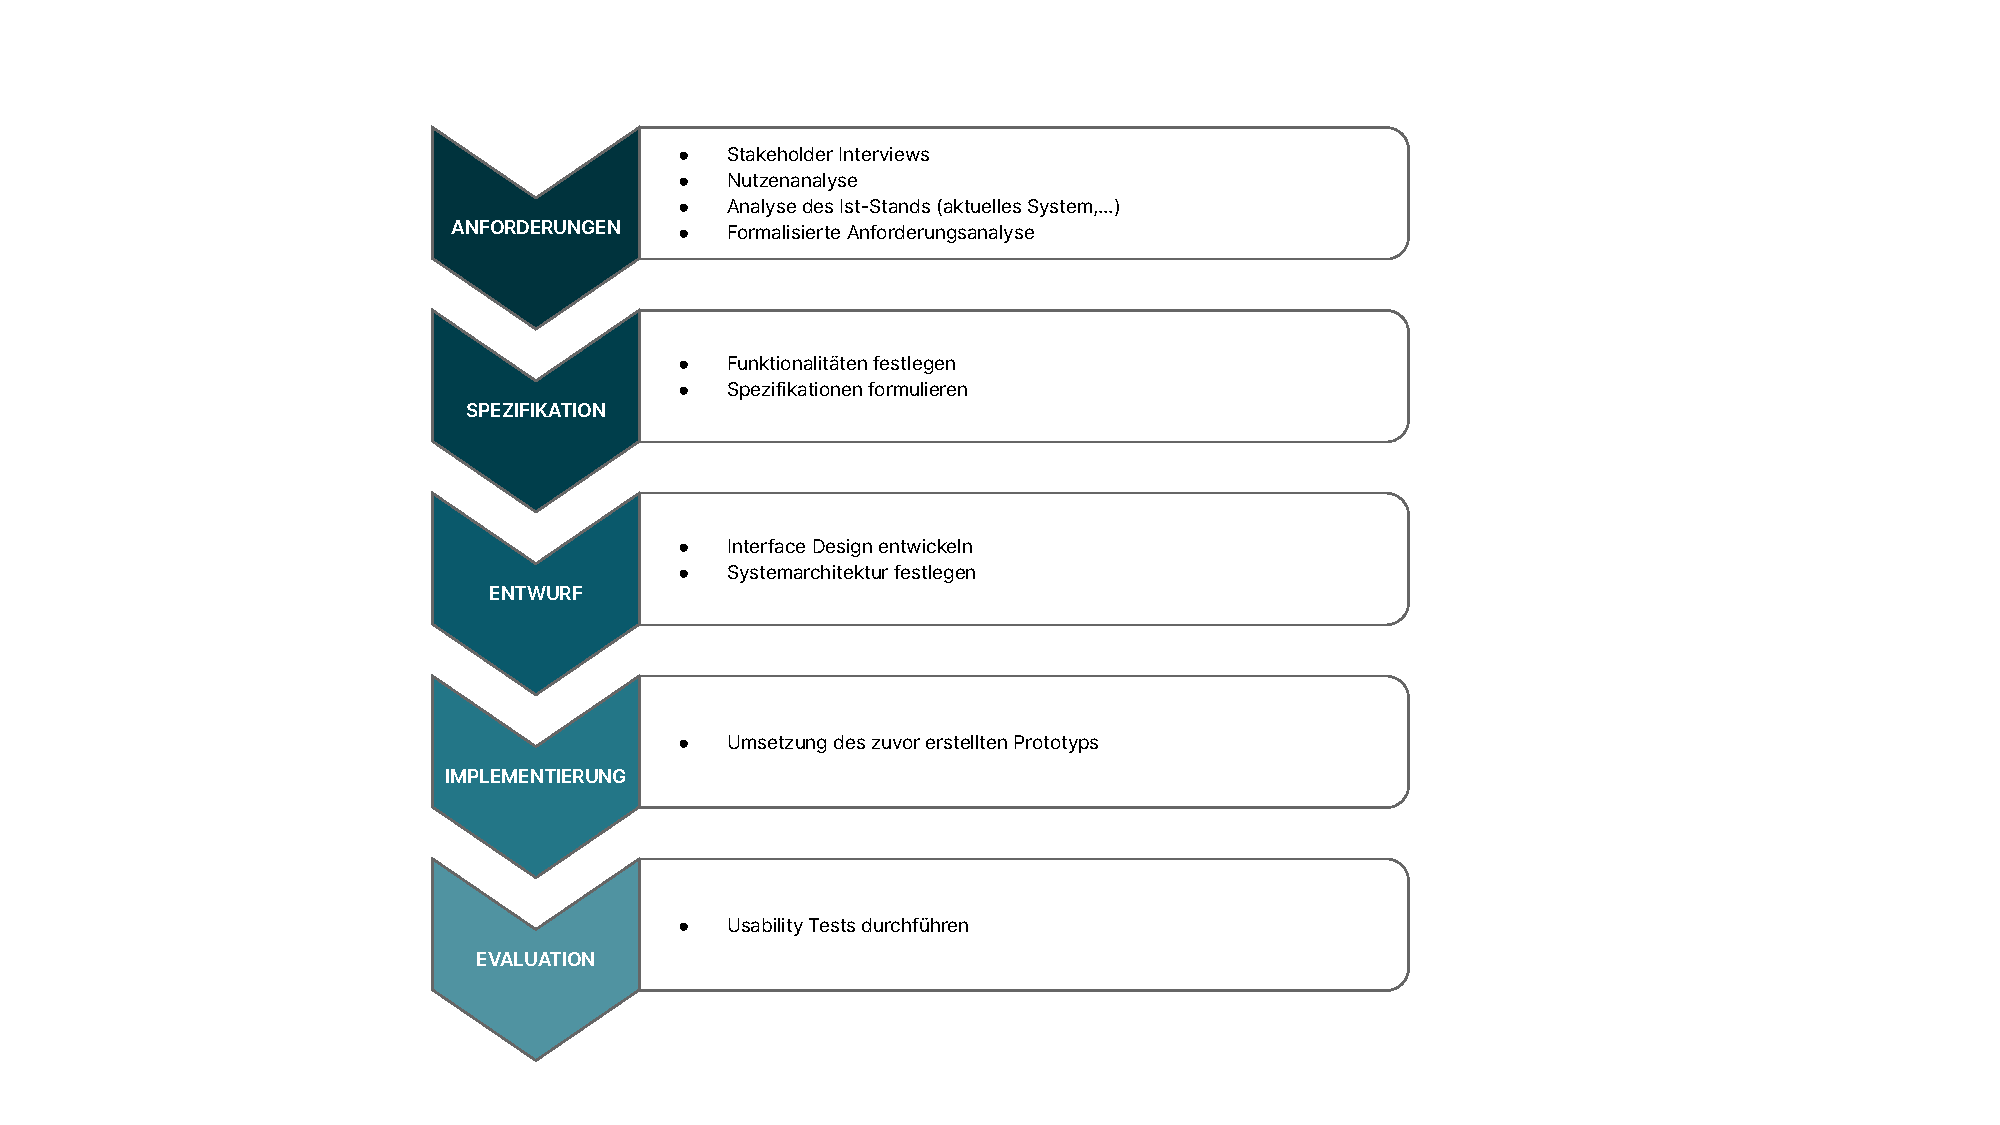
\includegraphics[scale=0.6]{Bilder/Vorgehensmodell.pptx.pdf}
  \label{fig:schablone}
  \caption[Vorgehensmodell]{Vorgehensmodell}
\end{figure}

In der ersten Phase wurden die Anforderungen an das zu entwickelnde System erarbeitet und
verstanden. Die Erkenntnisse dieser Phase sind in Kapitel \ref{chapter-analyse} zu finden.
\ref{chapter-analyse} beantwortet unter anderem auch die Forschungsfragen F1 und F2. Durch die
Interviews mit den Stackholdern konnten die zentralen Schwierigkeiten des Ausleihprozesses
festgestellt werden. Foglich wurden die Notwendigkeiten der angedachten Anforderungen mithilfe der
Interviews überprüft und ergänzt.

In der Spezifikationsphase werden die Anforderung an das System weiter spezialisiert
(\ref{chapter-konzept}). Daher wurden Funktionalitäten entsprechend den Anforderungen entwickelt und
in einer priorisierten Featureliste festgehalten. Anschließend wurde die Systemarchitektur, für das
Back-end, aufbauend auf den Anforderungen und damit einhergehenden Frameworks ermittelt. Darüber
hinaus wurde für das Front-end in der Entwurfsphase das Interface-Design erarbeitet
(\ref{chapter-design}). Hierbei wurde durch Usability Tests ein iteratives Vorgehen ermöglicht.

Die Implementierungsphasen umfasst die eigentliche Umsetzung des Reservierungstools
(\ref{chapter-implementierung}). Hierbei wurden die in der Konzeptionsphase festgelegten Frameworks
genutzt. \ref{chapter-dialogbeispiel} präsentiert das realisierte System anhand von
Dialogbeispielen.

In der abschließenden Phase wurde das realisierte System mithilfe von Interviews und Umfragen
evaluiert (\ref{chapter-evaluation}). Die Ergebnisse der Phase beantworten Forschungsfrage F3 und
geben Aufschluss über die Wirksamkeit des entwickelten Systems. Im Anschluss gibt
\ref{chapter-fazit} einige Perspektiven über offene Punkte und die mögliche Weiterentwicklung des
Systems.